\documentclass[12pt,a4paper]{article}

% Encoding
\usepackage[utf8]{inputenc}
\usepackage[T1]{fontenc}

% Page layout
\usepackage{geometry}
\geometry{a4paper,left=2.54cm,right=2.54cm,top=2.54cm,bottom=2.54cm}

% Font - Arial (LSE requirement)
\usepackage{helvet}
\renewcommand{\familydefault}{\sfdefault}

% Spacing
\usepackage{setspace}

% Bibliography
\usepackage[
backend=biber,
style=apa,
url = false,
doi = false,
isbn=false,
]{biblatex}
\addbibresource{bibliography.bib} %Imports bibliography file
\usepackage[hidelinks]{hyperref}

% Headers - candidate number (LSE requirement)
\usepackage{fancyhdr}
\setlength{\headheight}{14.5pt}
\pagestyle{fancy}
\fancyhf{}
%\rhead{\small Candidate Number: XXXXX}
\rfoot{\thepage}
\renewcommand{\headrulewidth}{0pt} %Links in-text citations to references

%Fix hbox warning
\sloppy

% Misc
\usepackage{graphicx}
\usepackage{booktabs}
\usepackage{appendix}

%Floating tables- "H" keeps them in place
\usepackage{float}

%For Turkiye "u"
\DeclareUnicodeCharacter{0307}{}

\begin{document}

\begin{doublespace}
% Cover page - Moodle requirement
\thispagestyle{empty}
\pagenumbering{gobble}                          % suppress page numbers
\begin{center}
    \vspace*{2cm}
    {\large GV499 Dissertation\\
    MSc Public Policy and Administration \\
    Department of Government\\
    London School of Economics}\\
    \vspace{2cm}
    {\Large\textbf{Captured by Design: Central Bank Independence as Structural Regulatory Capture}}\\
    \vspace{2cm}
    Candidate Number: XXXXX\\
    \vspace{0.5cm}
    Word Count: XXXXX\\
    \vspace{0.5cm}
    \today
\end{center}
\newpage

% Abstract
\section*{Abstract}
\vspace{\baselineskip}

My abstract goes here

\newpage



\tableofcontents
\newpage

% Double spacing - Moodle requirement

\pagenumbering{arabic}                          % page numbers start here
\setcounter{page}{1}
%\input{sections/introduction}
%\input{sections/literature}
%\input{sections/theory}
%\input{sections/empirical}
%\input{sections/conclusion}

%If you getg sick of the compiling extra files on Positron,
%motify settings.json in positron:
%    "latex-workshop.latex.autoClean.run": "onBuilt",
 %   "latex-workshop.latex.clean.method": "glob",
 %   "latex-workshop.latex.clean.fileTypes": [
 %       "*.aux", "*.bcf", "*.bbl", "*.blg", "*.idx", "*.ind", "*.lof", "*.lot", 
 %       "*.out", "*.run.xml", "*.toc", "*.acn", "*.acr", "*.alg", "*.glg", "*.glo", 
 %       "*.gls", "*.ist", "*.fls", "*.log", "*.fdb_latexmk", "*.synctex.gz", "*.synctex"
 %   ]




\newpage
\section{Introduction}

%Start with the Federal Reserve ruling

The interests of the financial sector are baked into institutional and legal definitions of central bank independence. These interests originate in the epistemological assumptions of the economics literature through the social objective functions utilized in the theoretical models (the ``conservative central banker") and empirical measurement of de jure central bank independence. The assumptions are transmitted, through personnel and discourse, into consistent blockage of legislative revision of the Fed's dual mandate. The end result is a system that reflects regulatory capture without requiring explicit coordination or lobbying among firms; private interests instead only have to promote inaction, and they can do so solely through their influence in the broader market.

The broader point: We build an argument that the economics literature that juswtifies central bank independence bakes in the preferences of the financial sector, and these papers have had an important epistemological influence on policymaking.

\section{Background and Theory}


\subsection{Economics Central Bank Independence Literature}

I begin by providing a more precise definition of central bank independence (CBI). \textcite{debelle_how_1994} distinguishes two core types of CBI: goal and instrument independence. Instrument independence handles the actual implementation of monetary policy to achieve those goals. When a central bank has instrument independence, is it able to utilize the tools of monetary policy to best achieve preset goals independently from political influence. In such a system, a political agent, such as the legislature or a president, is unable to influence the decision-making process for choosing which tools to use and how. For instance, if a central bank has instrument independence, a president cannot use their political influence to coerce a central bank into lowering interest rates, even if the president believes this is the best way to achieve the goals of monetary policy. If a central bank has goal independence, it has the power to choose what objectives it is attempting to achieve with its instruments. It can make judgements about what the most desirable economic outcome is, and then it can use its instrument independence to achieve these objectives. 



The Federal Reserve's institutional arrangement can help us distinguish these two forms of independence. Federal Reserve Chair Jerome \textcite{powell_panel_2023} applied Debelle and Fischer's framework to the Fed. In the 1977 amendment to the Federal Reserve Act, Congress established that the Federal Reserve has a tripartite mandate to achieve the goals of ``maximum employment, stable prices, and moderate long-term interest rates" through its monetary policy. The Federal Reserve coloquially refers to this as the ``dual mandate" of stable prices and maximum employment, dropping the moderate long-term interest rate component because of its ``redundancy" \parencite[15]{downey_our_2025}\footnote{I will address this further in my analysis section}. Powell then argues that ``The existence of the dual mandate reflects the fact that the Federal Reserve's monetary policy independence corresponds to operational, or instrument, independence, rather than goal independence." 

%In this paper, when I refer to central bank independence (CBI), I am referring to instrument independence alone. I will explicitly distinguish goal and instrument independence when necessary as I construct my argument.


The theoretical foundation for central bank independence in the economics literature lies in a few seminal works.  \textcite{kydland_rules_1977} were the first to apply the time-inconsistency and credible commitment public policy problem to the inflation-unemployment tradeoff detailed in economics literature. In brief, in a model economy with rational agents and a government seeking to maximize some ``social objective function," governments will naturally have a temptation to implement a surprise expansionary (inflationary) policy that temporarily pushes down unemployment \parencite[473]{kydland_rules_1977}. Rational agents predict this action, so they set their inflation expectations higher, meaning that the surprise action the government would implement would trigger even higher inflation. This principle makes credible commitment by governments challenging, so the end result is heightened inflation expectations from agents. Inflation becomes anchored at a level that is higher than what the social objective function deems optimal.

\textcite{barro_rules_1983} apply this logic directly to monetary authorities. First, note that they (along with much other theoretical literature on monetary policy) assume that monetary policy is neutral in the long-run. This principally means that while the amount of currency in circulation may increase with expansionary monetary policy, the relative price between goods should, in theory, not change after a change in monetary policy \parencite[49-50]{downey_our_2025}. Given this, \textcite{barro_rules_1983} suggests that monetary policy can only reap benefits if there is a short-run surprise, before prices can readjust. However, rational agents incorporate this in their inflation expectations, pushing up inflation without reaping any rewards if monetary policy is conducted under discretion. While a central bank may seek to preserve its reputation, thereby creating some credibility regarding its policies, this is only a partial substitute. \textcite{barro_rules_1983} argue that the optimal setup is a central bank that is entirely constrained by rules, thereby establishing credibility and anchoring inflation expectations of agents. \textcite[1177]{rogoff_optimal_1985} provide several possible solutions, including appointing a ``conservative central banker" who is ``known to place a greater weight on inflation stabilization" than the general public will suggest. In particular, Rogoff's conservative central banker ``places a larger weight on inflation relative to employment stabilization" \textcite[2]{romelli_trends_2024}. They will be less tempted to implement inflationary policy, and rational agents set inflation expectations lower as a consequence. While they acknowledge that this may not be theoretical optimal, the conservative central banker argument underpins much of the empirical literature defending CBI.

Central bank independence has become the dominant form of monetary policymaking around the world. This process occurred over a period of decades following the end of World War II, but much modern analysis of CBI begins with the late 1970s/early 1980s Federal Reserve. During the stagflation episode of the late 1970s, where oil supply shocks meant high inflation occurred during a period of heightened employment, Paul Volcker assumed became Fed Chair in 1979. He chose explicitly to prioritize combatting inflation over unemployment, despite pressure from President Reagan to lower interest rates. During his tenure, the Fed raised interest rates significantly, putting the economy in a recession while simultaneously bringing down inflation. This episode is frequently referenced in the economics literature for two reasons. First, it serves as a simple empirical example of the time inconsistency problem, where a misguided politician wanted interest rates lower than what was optimal. Second, the Federal Reserve technocrats used their special expertise to successfully combat an inflation episode. Even though there was short-term pain in the economy, the US reaped the long-term benefits, providing legitimacy to the technocrats of central banks holding unique, strong monetary policy powers. Under these assumptions, CBI became the institutionally accepted arrangement for central banking. 


\subsection{Alternative Literature on CBI}

\label{sec:political_sci_lit}

I now turn to the alternative literature on CBI. While the previous section describes the core concepts that are embodied in the traditional and institutional discourse of monetary policy, there is a well established body of work questioning these assumptions. It is worth noting that these materials come from academics of a variety of different backgrounds, not just political scientists. I focus on academic pieces whose content differs from the assumptions made in the previously discussed economics literature.  In later sections, I will apply these critiques to the economics literature, emphasizing how they are neglected, and how the economics literature, rather than the political science literature, dominates policymaking. I begin with the big picture, institutional literature on CBI, and then I zoom onto individual actors.

Literature has questioned the narrative about the proliferation of central bank independence being tied to economic performance and the time inconsistency problem. One could imagine a situation where politicians could pass irresponsible economic policy, like large tax cuts or direct payments to citizens, immediately before elections. The academic, time-inconsistency argument alone becomes insufficient to justify the rise in the power of central banks. Political scientists point to central banks as institutions, and central bank independence as political decisions. 


The technocratic legitimacy argument, where unbiased technocrats of central bank produce more optimal policy than politicians, has been criticized by political scientists. Built into the time inconsistency problem, as previously described, is an assumption that politicians should not be entrusted, primarily because of their incentives to stimulate the economy before elections and because of their lack of expertise on monetary policy. This assumption assumes that the technocrats within a central bank are both unbiases and have sufficient expertise to guide monetary policy. 

\textcite{wansleben_rise_2023} describes this legitimacy as an attempt to establish bureaucratic power. They also handle how price stability alone may not be solely a mechanism that's pro finance. The Fed has engineered expansionary policies to benefit finance as well.

Literature on central banking is quite thorough, and it is impossible to fully encapsulate all of the different arguments. Thus, I focus on the biases regarding monetary policymaking, from the policymakers themselves to the institution-building of the Federal Reserve.

%The default of what is apolitical- there is some political decision that was then deemed apolitical.
%Wanslaben and the fed as institution building
% Rational fiction- missing politics of CBI
%CBI as a political construct. 
%Finance has grown as a percent of gdp significantly since the establishment of CBI- and

%%%Central bankers are biased: CBI is rational fiction

\subsection{Regulatory Capture}

Conceptualizations of regulatory capture are often rooted in the seminal work by \cite{stigler_theory_1971}. 

\subsection{Non-Interactions of Economics and Political Science Literatures}

%%%The rational fictions to the de facto literature; 

\section{Methodology}

\subsection{Research Design}

\subsection{Causal chain and evidentiary tests}

\subsection{Rival hypothesis}

\section{Analysis}

\subsection{Epistemological Assumptions in the Economics Literature}


\subsubsection{Theoretical Economics Modeling}
%Normative Loading
%The first evidence for structural regulatory capture should be in the epistemic environment that CBI is built upon. In particular, there is a significant economics literature defending CBI. Many policymakers in central banking that this is a well-established consensus, and few mainstream policymakers openly criticize this consensus. If central bank independence reflects the interest of finance, then, principally, those interests should be reflected in assumptions that govern empirical and theoretical analysis of central banking. 

%

%%%We probably do want to discuss the general findings of chapter 3 from Downey

%Dissect page 479 and 480; there is a general push and pull 

%Unemployment has a lasting benefit for those who get jobs.


The theoretical principles for central bank independence, as previously discussed, are rooted in the time inconsistency problem from the time inconsistency problem, originally presented by \textcite{kydland_rules_1977}.  They begin their presentation of the solution with an ``agreed-upon social objective function" that is ``assumed to exist" \parencite[475]{kydland_rules_1977}. Yet, it is not always apparent in economics literature why inflation should be included in some monetary policy social objective function in the first place. \textcite[52]{downey_our_2025} notes how previous Fed Chair Ben Bernanke states, ``In the long run, the central bank can affect only
inflation, and not real variables such as output." After all, if the price for of goods increases, but buying power also increases (wages increase), consumers can purchase just as many goods as before. \textcite[58-61]{downey_our_2025} critiques the idea that there are costs to society of inflation.\footnote{In the interest of time, I generally ignore hyperinflation in this essay, but it is worth noting that there are plenty of historical examples of non-dependent central banks not experiencing hyperinflation, including the United States in the three decades following WWII.} In particular, the Federal Reserve meets the price stability component of its dual mandate by targeting 2\% inflation, measured primarily through the ``core" (excluding food and gas) Personal Consumption Expenditures index produced by the Bureau of Economic Analysis. Measuring inflation through a single measure creates problems. Different socioeconomic groups consume differently, and a single measure misses this heterogeneity. 

I emphasize two forms of heterogeneity in the impact of inflation. First, how indices define the ``relative" basket of goods used to estimate overall price increases is incredibly important. Federal Reserve officials emphasize the role that inflation can play for the poor, where families barely have enough consumption power to make ends meet, and they use this to justify their monetary policy decisionmaking. If a family is living paycheck-to-paycheck, and prices increase more than their paycheck, they may be unable to pay for essential goods and services. Meanwhile, wealthier families can use their savings or investment income the minimize the damage of inflation. Thus, it would be useful for the Federal Reserve to measure the erosion of consumption power for the poor and the influence of policy on this erosion. This, currently, is not part of the Federal Reserve's objectives.

Setting aside this heterogeneity, there is a real, measurable cost to inflation for creditors (particularly banks) relative to debtors. A core feature of bank intermediation is maturity transformation, where banks take cash (deposits) and other short-term investments and make long-term loans (mortgages, corporate loans, etc...). These loans generally have a fixed interest rate. If inflation spikes, the real value of these loans falls; each dollar a debt repays the creditor becomes worth less than when it was borrowed. Here, an aggregate measure of inflation becomes more appropriate to use. Banks distribute money into the entire economy, so the average value of a given dollar influences the ability for banks to continue lending, based on the recouped gains from previous loans. Given that there are varying costs to inflation for different interest and demographic groups, ``inflation has significant redistributive effects" \textcite[256]{posen_declarations_1995}.


Given this, it is clear that how we measure inflation, and why we care about inflation, varies significantly. Yet the theoretical literature on monetary policy begins modeling under the core premise that there is some social objective function that reflects the aggregate preferences of society. In particular, \textcite[480]{kydland_rules_1977} describe a ``socially preferred inflation rate is zero, which seems consistent with the public's preferences," and ``a more informed public might prefer some  positive or negative inflation." \textcite[103]{barro_rules_1983} acknowledge ``distortions from income taxation, unemployment compensation, and the like," yet ignores these distortions in the interior model. While, they think ``of the monetary authority’s objective as reflecting the preferences of the “representative’ private agent," they ``express this objective as a function of actual and expected rates of inflation" \parencite[102]{barro_rules_1983}. \textcite{rogoff_optimal_1985} extends the modeling implications that are predicated off having one uniform, socially optimal inflation rate. The premise of the conservative central banker is a central banker who is more inflation-averse than the public. Yet, Rogoff leaves an underlying question unanswered: How might a central banker obtain this anti-inflation bias? What influences might lead to such an outcome?

One possible answer is that central bankers, as technocrats, are influenced by the economics literature and the ``facts" of monetary policy. They understand technically what monetary policy is and why it matters, far more than the public or political figures. The economics literature itself thus becomes self-reinforcing: central bankers believe the models of economics literature and believe they are optimal for society, so they follow them. However, the literature described in \ref{sec:political_sci_lit} addresses both the biases of central bankers intrinsic in policymaking and the limits of technocratic justification for the democratic delegation of monetary policymaking. 

A second possible answer is that special interest groups who uniquely benefit more from lower inflation relative to the rest of the public can help enforce central bank independence. In particular, \textcite[256]{posen_declarations_1995} argues that increasing CBI "is taken to be equivalent to increasing the relative weight of price stability over employment goals in the monetary authority's utility function," and that this "conforms with the conservative central banker of Rogoff (1985)." Posen identifies this interest group as the financial sector: ``the financial sector is uniquely positioned to provide that support, and central banks have been most independent where that support has been strongest" \parencite[254]{posen_declarations_1995}. 

%%%We can mention IOER and negative rates if we want to
The expansion of monetary policy's power, combined with the low interest rate environment since 2008 complicates the picture that finance exclusively benefits from the weighting of price stability over the employment in monetary policy goals. Large scale asset purchases are the immediate example of this, because ``by recapitalizing the financial sector and not the broader economy, QE had a political multiplier effect that enhanced the political influence of banks at the expense of ordinary citizens" \textcite[738]{adolph_missing_2018}. The core takeaway from this subsection is not that finance uniformly benefits from tight monetary policy. Instead, the development of the theoretical literature that justifies central bank independence, and thus, modern western monetary governance, is predicated on a model that explicitly overvalued a normative assumption that benefited financial institutions. Their interests were modeled as the interests of finance through the development of the ``conservative central banker," while the complexities of the distributional consequences of inflation were left out of monetary policy. In the next section, I demonstrate how the assumptions, which encoded the interests of finance, heavily influenced the empirical literature measuring the efficacy of CBI.
%%%%Note that the de facto literature does not address the political criticisms of QE- which is a necessarily expansionary policy, and policy that uniquely benefits financial institutions. We should unpack that point a bit more- that the mandate has changed who benefits from X.


%Let's use the term normative loading.

%Much of this literature is predicated on the idea that monetary policy is neutral in the long-run \parencite{downey_our_2025}.



\subsubsection{Empirical Evidence and CBI Indices}

%Brainstorm: The central bank independence discussion- post-COVID inflation spike. Updating on past performance- CBI is tougher to justify after this spike. This is also a post-2020 episode; the discourse around the CBI had to change around inflation- but it really didn't.

%Weiss paper on enlightenment model of public policy- Keynes paper 

%You can narrate the history of the literature and CBI

%Hofer- QE and capture is interesting, but IDK if I have space.


Economics literature has attempted to measure the influence of the aforementioned theoretical models through empirical analysis. Regarding both goal and instrument independence, it can be difficult to measure the level of influence of political figures on central bank decisions. Thus, many empirical papers distinguish between ``de jure" and ``de facto" indepndence. While de facto analysis attempts to analyze the personal influence of politics on central banking, de jure measures ground themselves in the law surrounding monetary governance, from appointment of central bank officials to the laws establishing the goals of monetary policy. I emphasize de jure independence in this paper because the assumptions in determining what an ``independent" central bank truly means are informative. These assumptions are explicitly described in the methodologies of de jure papers, but because de facto papers measure things like political influence, they have less commentary on the central banking institutionally. I describe the influence these papers have on monetary policy discourse in the next section.

Empirical measurement of de jure CBI generally involves simplifying the laws governing a central bank into an index. Authors study different components of central bank governance, and determine the degree to which the law describes an independent central bank. Indices define perfect de jure CBI as ``1" and complete de jure central bank dependence as ``0." Arguing for the merits of a given index or strategy is beyond the scope of this paper, but they all share a basic theoretical basis in the arguments initially presented by \textcite{kydland_rules_1977}, \textcite{barro_rules_1983}, and \textcite{rogoff_optimal_1985}. These empirical papers generally find one result, namely that the politicization of monetary policy raises inflation without boosting economic growth \parencite[4]{posen_introduction_2025}. 

%I feel like this is an important paragraph, so we want to return to it
In the coming paragraphs, I will analyze various de jure CBI papers and argue that a core feature of this literature is the conflation of goal and operational independence. Under the \textcite{fischer_central-bank_1995} model, even though instrument independence is optimal, the goals of monetary policy should be entirely set through political processes. The type of goals a central bank is set to achieve should thus not be relevant to a CBI index if that index is principally measuring instrument independence. In particular, a codified ``price stability" target is often incorporated as part of the optimal arrangement of an independent central bank. This may be optimal for achieving the conservative central banker vision of monetary policy, but the definition itself has little to do with how independent a central bank is.

Some of the most influential works on de jure CBI are \textcite{bade_central_1988}, \textcite{alesina_credibility_1988},  \textcite{grilli_political_1991}, and \textcite{alesina_central_1993}. \textcite{alesina_credibility_1988} builds on a methodology developed by \textcite{bade_central_1988} to create one of the earliest measures of de jure independence. They decompose forms of independence into ``political" and ``financial" independence. Political independence generally deals with insulation of central bank officials from political processes (like appointment and firing protections and the government approval of monetary policy decisions) to achieve monetary policy objectives, while financial independence emphasizes if the central bank is legally obligated to finance the government. While \textcite{bade_central_1988} consider both forms of independence, \textcite{alesina_credibility_1988} focuses almost exclusively on political independence. The codified goals of monetary policy are not explicitly included in these definitions. 

This changes with \textcite[366]{grilli_political_1991}, where ``political indepencence" is defined as ``the capacity to choose the final goal of monetary policy". This is distinct from economic independence, or the ``capacity to choose the instruments with which to pursue these goals". Political independence can be mapped as a precursor to \textcite{fischer_central-bank_1995}'s goal independence, while economic independence is similar to instrument independence.

\textcite{alesina_central_1993} produces a statistical model measuring how different levels of CBI influence economic variables like output and inflation, based on an average measurement of the degree of independence described by \textcite{alesina_credibility_1988} and \textcite{grilli_political_1991}. They find that ``while central bank independence promotes price stability, it has no measurable impact on real economic performance" \textcite[151]{alesina_central_1993}. Additionally, there is ``a near perfect negative correlation between inflation and central bank independence" \textcite[153]{alesina_central_1993}. This finding has been cited thousands of times throughout the economics literature, and as we will discuss in section XXX, has made a large impact on policymakers at the Federal Reserve. Most importantly, \textcite{alesina_central_1993} accept the inclusion of ``the 'price stability' objective is explicitly and prominently part of central bank statute" in \textcite[153]{grilli_political_1991}'s work as an essential part of the definition of political independence.


%However, it is worth noting that these papers are not complete in their analysis, and they all recognize their own limitations. In particular, measuring the operational independence that exists between a central bank in its decisions and political authorities is intrinsically different to measure. The human relationships between these figures, and the ``true" justifications why certain decisions were made, are not always apprent. Influence is frequently tied to actions outside public knowledge, and it is impossible to know the full extent of influence. Furthermore, the stability and power of the legal institutions that enforce these laws greatly influence how politics influence central banking, and this influence is not detectable in a de jure CBI index.

%This is rough. Clean it up
At approximately the same time, \textcite{cukierman_measuring_1992} produced an expanded index on de jure CBI. They included more countries and more components than previous works, and as a consequence, this work has been repeatedly extended and enhanced by more modern economics literature, including, but not limited to, \textcite{romelli_political_2022}, \textcite{romelli_trends_2024}, \textcite{dincer_central_2024}, and \textcite{garriga_revisiting_2025}. In other words, \textcite{cukierman_measuring_1992}'s methodology is the root of most modern measures of de jure CBI. Crucially, \textcite{cukierman_measuring_1992} no longer distinguished between the political and economic independence components when building its measures of de jure independence. However, they continue to include objectives component of independence as a crucial component of the index. It is also linked explicitly back to the previously described theoretical literature: ``In \textcite{rogoff_optimal_1985}'s terminology, the objectives variable measures the strength of the 'conservative bias' of the bank's charter" \parencite[357]{cukierman_measuring_1992}.



%adrian, \textcite{dincer_central_2014},

%Hofer also analyzes QE- something that these essays don't do. Note that.


Recall that the United States legally has a ``tripartite" monetary policy mandate which it coloqially refers to as its ``dual mandate."\footnote{While in practice this may not significantly alter monetary policy, the ability for the Federal Reserve to simply ignore a piece of the law compromises the principle of goal independence \parencite{downey_our_2025}.} That said, all of the aforementioned de jure measures of CBI code the Federal Reserve's monetary policies as the ``dual mandate." The underlying problem for these indices is that if Congress decided to revise the Federal Reserve's mandate, this decision would alter the Federal Reserve's CBI score. For instance, if Congress eliminated the unemployment component of the dual mandate, the United States CBI score would universally increase. This intrinsic action does not influence, definitionally, goal \textit{or} instrument independence, because Congress would still be responsible for setting monetary policy objectives (goal dependence) and would not have changed its ability to influence individual policy decisions (instrument independence). However, the measurement of CBI in every de jure index would significantly changed.


The conflation of goal and instrument independence has implications in the de jure measurement of CBI today. Using a comparison of the United States and T\"urkiye as a case study can be illuminative. ``The political system in T\"urkiye has been rapidly centralizing around the executive branch of the state, while the power of independent state institutions eroded" since 2011 \parencite[62]{demiralp_erosion_2019}. The Economist Intelligence Unit reported a significant decline in its measure of democracy in T\"urkiye from a peak of XXX in XXX to XXX in XXX. This trend has coincided with President Erdo\u{g}an increasing pressure on the CBRT to maintain low interest rates \parencite{gurkaynak_consequences_2023}. 

Inflation rapidly spiked in 2018 in T\"urkiye, particularly following a constitutional reform that dramatically increased President Erdo\u{g}an's political power. Following the reform, the CBRT fully implemented President Erdo\u{g}an's unorthodox view that lower interest rates reduces (rather than increases) inflation, on average. A variety of papers, from XXX to XXX, have attributed the political pressure on the CBRT to the rapid spike in inflation that the Turkish economy has experienced, particularly following the COVID pandemic. Figure \ref{fig:turkishinflation} displays Turkish inflation from 1990-2024. Between 2003 and 2016, Turkish inflation remained below ten percent. From 2017 on, the rate rose to above 10 percent, and between 2020 and 2022, the rate spikes from 12 to 72 percent. 

\begin{figure}[h]
\centering
\caption{Turkish Inflation, 1990-2024}
\label{fig:turkishinflation}
\begin{minipage}{0.65\textwidth} % choose width suitably
\centering
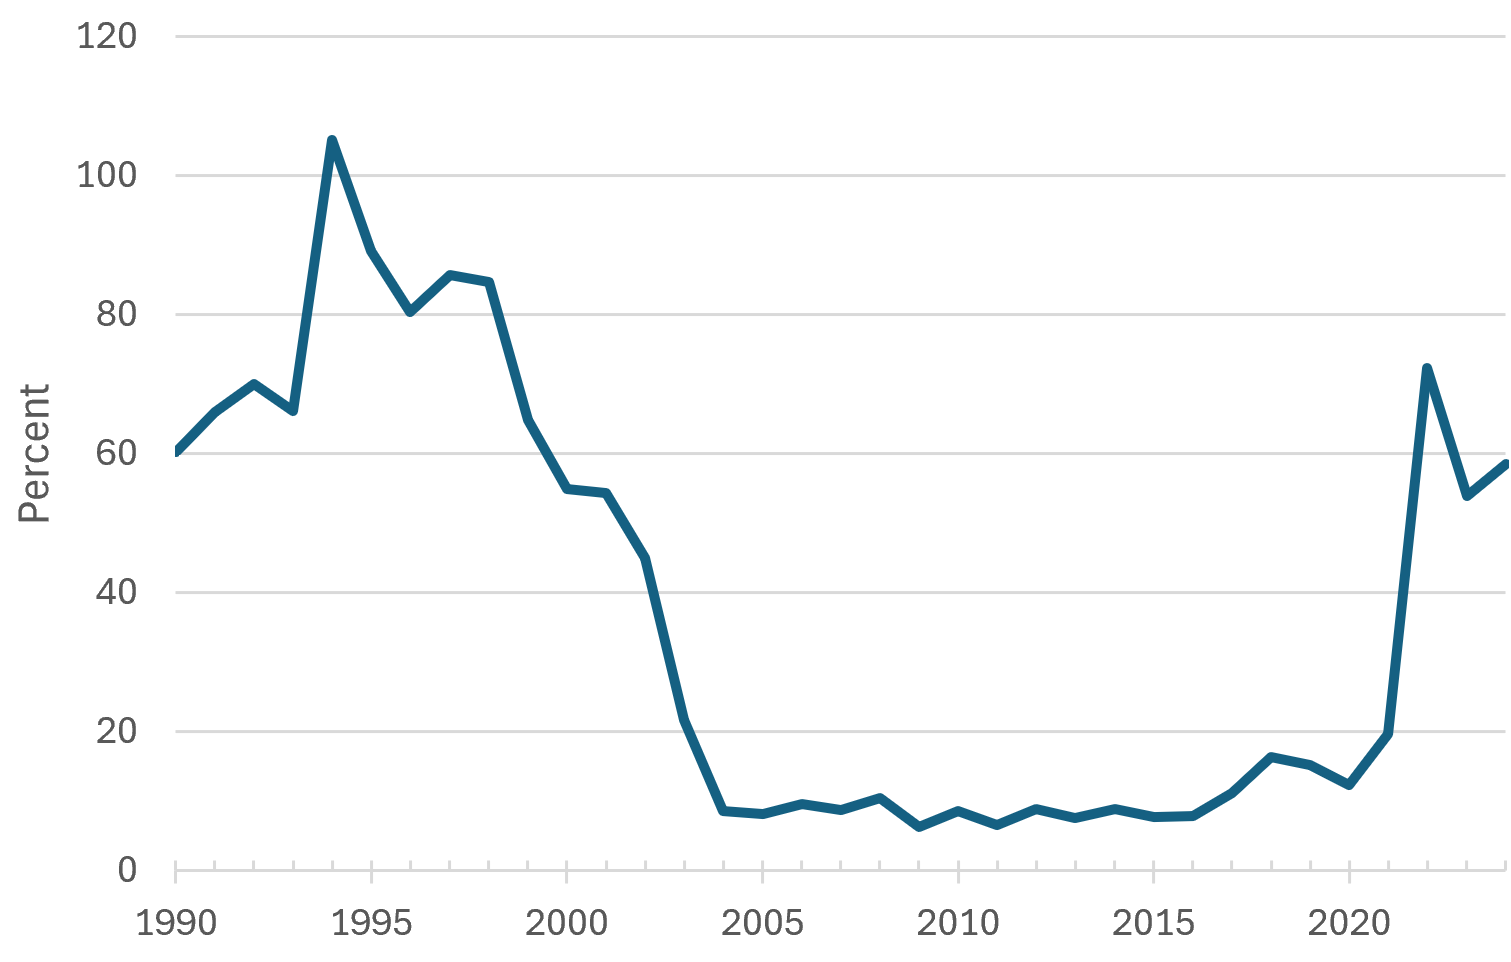
\includegraphics[scale = 0.8]{Turk Inflation.png}
\footnotesize{\textit{Source:} World \textcite{world_bank_inflation_2026}\par} 
\end{minipage}
\end{figure}

A variety of commentators have described the Turkish situation as evidence about the importance of the erosion of CBI, and they have applied it to the American context. \textcite{posen_introduction_2025} attaches this spike to President Erdo\u{g}an removing and replacing central bank governors who do not support his views for monetary policy. \textcite[530]{gurkaynak_consequences_2023} cite the decay of CBI in T\"urkiye as the ``only plausible answer" for the lack of a strong anti-inflationary response to the CBRT. Such firings serve as a method of eroding operational independence for the CBRT, where individual interest rates become heavily biased by the executive authority, not the technocrats running the CBRT. While \textcite{jeddy_cautionary_2025} warns that President Trump's political pressure on the Fed may result in a similar story to T\"urkiye. However, to date, President Trump has been unsuccessful in removing Federal Reserve policymakers from office. With some caveats, the Federal Reserve's ``institutional strength is well established," meaning that the Turkish erosion of CBI did not occur in the United States, despite President Trump's pressure \textcite[542]{cakmakli_financial_2024}.
%%%Gonna need to revise this one- talk about the supreme court

Despite this, the conflation of goal and instrument independence within the de jure measures of central bank independence results in T\"urkiye having a uniformly \textit{higher} score than the Federal Reserve.  First, it is worth noting that de jure indices, despite being largely based on the core framework from \textcite{cukierman_measuring_1992}, do make a series of subjective coding and methodology decisions. The way that the de jure indices utilized in this paper differ are summarized in table \ref{tab:cbi_index_comparison}. I cite these differences not to argue which methodology is ``best," but rather to establish that there is some academic debate ongoing about the most appropriate methodology for a de jure CBI index, and different measurement strategies are already being developed in the literature.  Despite all of the different methodologies, all three papers include the goals of a central bank as an integral part of their measurement schemes.\footnote{The component data for \textcite[399]{dincer_central_2024} was unavailable, but the methodology confirms the inclusion of an ``Objectives Component" which studies the ``objectives of the central bank, including an emphasis on price stability versus other goals. Additionally, while \textcite{grilli_political_1991}'s index was replicated and updated by \textcite{romelli_trends_2024}, there is no published version of \textcite{bade_central_1988} available}.

%Because coding laws is a subjective process requiring decisions on a case-by-case basis, and deciding which types of laws to include in analysis is also a subjective proces, papers that have attempted to extend \textcite{cukierman_measuring_1992} can end up with different index values for the same country and time.

\begin{singlespace}
\begin{table}[H]
\centering
\caption{Comparison of De Jure Central Bank Independence Indices}
\label{tab:cbi_index_comparison}
\begin{tabular}{p{3.2cm}p{3.2cm}p{3.6cm}p{3.6cm}}
\toprule
 & \textcite{garriga_revisiting_2025} & \textcite{romelli_trends_2024} & \textcite{dincer_central_2024} \\
\midrule
Base tradition & CWN & GMT + CWN integrated & CWN \\
\addlinespace
Dimensions & 4 & 6 (adds financial independence, reporting/disclosure) & 4 (8 components) \\
\addlinespace
Disaggregated criteria & $\sim$CWN's 16 & 42 & CWN's 16 \\
\addlinespace
Coverage & 192 countries, 1970--2023 & 155 countries, 1923--2023 & 120 countries, 1800--2021 \\
\addlinespace
Aggregation & Unweighted + weighted & Weighted sub-indices & LVAU / LVAW / LVES / LVESX \\
\addlinespace
Distinctive feature & Broadest country coverage & Most criteria; new dimensions & Longest history; ML validation \\
\bottomrule
\end{tabular}
\smallskip
\begin{minipage}{\linewidth}
\footnotesize\textit{Notes:} All three are \textit{de jure} indices derived from the Grilli, Masciandaro \& Tabellini (1991, ``GMT'') and Cukierman, Webb \& Neyapti (1992, ``CWN'') coding traditions. \textcite{garriga_revisiting_2025} codes four \textcite{cukierman_measuring_1992} dimensions (personnel independence, objectives, policy formulation, limits on lending). \textcite{romelli_trends_2024} integrates \textcite{grilli_political_1991} and \textcite{cukierman_measuring_1992} and adds financial independence and reporting/disclosure criteria. \textcite{dincer_central_2024} applies the CWN 16-criterion scale and adds a machine-learning validation layer.
\end{minipage}
\end{table}
\end{singlespace}

All of the aforementioned indices measure the CBRT as being more independent than the Federal Reserve. Tables \ref{tab:romelli_cbi}, \ref{tab:garriga_us_cbi}, and \ref{tab:dincer_cbi} show a comparison of how the United States Federal Reserve scores on de jure independence measures relative to CBI. At face value, this makes sense, given what these indices are measuring. The CBRT's mandate was revised following the Turkish currency crisis in 2001, and it was written to match the international norms of central bank independence that is now well established in countries around the world. Thus, if these indices were measuring ``how well a law chartering a central bank encapsulates the international norms associated with CBI," the Turkish laws fit perfectly.

However, these indices do not measure independence, for two reasons. First, these measures leave out the strength of the institutions enforcing the laws of the central bank. On paper, the de jure independence of the CBRT has not changed in recent years, yet the expansion of presidential power (and subsequent decline in democracy in Turkey) is left out. Indeed, while XXX mentions that there is a direct correlation between democracy and CBI, virtually all papers ignore this for practical puproses. It is worth noting that the expansion of the trend of CBI, as a political maneuver, was largely based on the understanding that CBI enhances the credibility of the party that establishes it. The US was at the core of the rapid growth of CBI, as it used its international influence to entice other nations to follow its lead. However, the laws in the US themselves do not reflect the broader independence that the Federal Reserve has, because despite these indices' findings, the US is simply seen as more independent than most other central banks. 



%https://www.brookings.edu/articles/challenges-to-independence-how-should-central-banks-respond-lessons-from-history/#:~:text=We%20have%20extensive%20evidence%E2%80%94across,electoral%20incentives%20make%20it

\begin{singlespace}
\begin{table}[H]
\centering
\caption{Central Bank Independence Scores: United States vs.\ T\"urkiye (2023), \textcite{romelli_trends_2024} }
\label{tab:romelli_cbi}
\begin{tabular}{lccc}
\toprule
\textbf{Index / Sub-index} & \textbf{USA} & \textbf{T\"urkiye} & \textbf{Gap} \\
 & \textbf{(2023)} & \textbf{(2023)} & \textbf{(T\"urkiye $-$ USA)} \\
\midrule
\multicolumn{4}{l}{\textit{CBIE Index}} \\
\quad Overall & 0.614 & 0.801 & +0.187 \\
\quad Board independence & 0.506 & 0.590 & +0.084 \\
\quad Policy independence & 0.700 & 0.800 & +0.100 \\
\quad \textbf{Objectives} & \textbf{0.250} & \textbf{1.000} & \textbf{+0.750} \\
\quad Lending restrictions & 0.938 & 1.000 & +0.063 \\
\quad Financial independence & 0.667 & 0.667 & \phantom{+}0.000 \\
\quad Reporting \& accountability & 0.625 & 0.750 & +0.125 \\
\midrule
\multicolumn{4}{l}{\textit{Comparison indices}} \\
\quad GMT Index (normalised) & 0.750 & 0.813 & +0.063 \\
\quad CWN Index (unweighted) & 0.808 & 0.909 & +0.101 \\
\quad CWN Index (weighted) & 0.735 & 0.867 & +0.132 \\
\bottomrule
\end{tabular}
\smallskip
\begin{minipage}{\linewidth}
\footnotesize\textit{Notes:} All scores are on a $[0,1]$ scale where 1 denotes maximum independence. Data sourced directly from sources referenced in the table. The bolded ``Objectives" sub-index from \textcite{romelli_trends_2024} measures the degree to which price stability is the sole or primary statutory mandate. GMT references the index first produced by \textcite{grilli_political_1991}, while CWN references \textcite{cukierman_measuring_1992}. Both were recoded and extended by \textcite{romelli_trends_2024}.
\end{minipage}
\end{table}
\end{singlespace}

\begin{singlespace}
\begin{table}[H]
\centering
\caption{Central Bank Independence Scores: United States vs.\ T\"urkiye (2023), \textcite{garriga_revisiting_2025}}
\label{tab:garriga_us_cbi}
\begin{tabular}{lccc}
\toprule
\textbf{Index / Sub-index} & \textbf{USA} & \textbf{T\"urkiye} & \textbf{Gap} \\
 & \textbf{(2023)} & \textbf{(2023)} & \textbf{(T\"urkiye $-$ USA)} \\
\midrule
\multicolumn{4}{l}{\textit{CWN Index}} \\
\quad Overall (unweighted) & 0.391 & 0.861 & +0.470 \\
\quad Overall (weighted)   & 0.475 & 0.899 & +0.424 \\
\midrule
\multicolumn{4}{l}{\textit{Sub-indices}} \\
\quad CEO independence        & 0.438 & 0.645 & +0.207 \\
\quad \textbf{Objectives}    & \textbf{0.400} & \textbf{0.800} & \textbf{+0.400} \\
\quad \textbf{Policy formulation} & \textbf{0.100} & \textbf{1.000} & \textbf{+0.900} \\
\quad Limitations on lending & 0.626 & 1.000 & +0.374 \\
\bottomrule
\end{tabular}
\smallskip
\begin{minipage}{\linewidth}
\footnotesize\textit{Notes:} All scores are on a $[0,1]$ scale where 1 denotes maximum independence. Data sourced from \textcite{garriga_revisiting_2025}, following \textcite{cukierman_measuring_1992} coding criteria. The Objectives sub-index measures the degree to which price stability is the sole or primary statutory mandate. The policy formulation component comprises who formulates monetary policy, the conflict resolution process, and the central bank's influence on the government's budgetary process.
\end{minipage}
\end{table}
\end{singlespace}


\begin{singlespace}
\begin{table}[H]
\centering
\caption{Central Bank Independence Scores: United States vs.\ T\"urkiye (2023), \textcite{dincer_central_2024}}
\label{tab:dincer_cbi}
\begin{tabular}{lccc}
\toprule
\textbf{Index} & \textbf{USA} & \textbf{T\"urkiye} & \textbf{Gap} \\
 & \textbf{(2021)} & \textbf{(2021)} & \textbf{(T\"urkiye $-$ USA)} \\
\midrule
\multicolumn{4}{l}{\textit{Legal independence indices}} \\
\quad LVAU (unweighted) & 0.698 & 0.844 & +0.146 \\
\quad LVAW (weighted) & 0.647 & 0.794 & +0.147 \\
\quad LVES (narrow) & 0.560 & 1.000 & +0.440 \\
\quad LVESX (extended narrow) & 0.736 & 1.000 & +0.264 \\
\bottomrule
\end{tabular}
\smallskip
\begin{minipage}{\linewidth}
\footnotesize\textit{Notes:} All scores on a $[0,1]$ scale where 1 denotes maximum independence. Values are 2021 country means from \textcite{dincer_central_2024}, Table 5. LVAU and LVAW are the unweighted and weighted aggregations of eight components following \textcite{cukierman_measuring_1992}; LVES is a narrow index covering policy formulation and objectives, and LVESX extends it with limits on lending to the government.
\end{minipage}
\end{table}
\end{singlespace}


Secondly, the objectives component definitionally does not measure CBI, and this significantly biases the indices. The `objectives" component gives the biggest gap between the two nations for \textcite{romelli_trends_2024} and the second most for \textcite{garriga_revisiting_2025}. While weighting schemes for developing the indices vary by author, there is consensus that having a price stablity mandate alone should weighted as substantially important when measuring de jure CBI. For instance, \textcite[4]{eijffinger_central_2026} describes how the \textcite{cukierman_measuring_1992} index ``considers the conservativeness of the central bank as defined by law" through determining the degree emphasis to which ``central bank law gives to price stability," and also that ``this aspect of the index should have been given much more weight" then \textcite{cukierman_measuring_1992} originally provided. 


This flies in the face of the theoretical distinction, which has been echoed by Federal Reserve institutional leaders, that the Federal Reserve serves at the leisure of the mandate Congress sets out for it. Consider, for instance, that Congress decided to pass a law that the Federal Reserve should prioritize reducing inequality in access to credit above its price stability mandate. Institutionally, nothing would have changed; the Fed would still have autonomy in deciding which tools at its disposal to use to accomplish this objective\footnote{Perhaps it could make a new lending facility providing credit for the opening of bank branches in underserved areas, as an example.} More directly, say that Congress argues that monetary policy should be constructed with the goal of serving the poor or middle class first, explicitly\footnote{They could emphasize using a basket of goods to measure inflation utilized by the poor, or to measure full employment, they could use slices of the economy that leave out the wealthy.} This normative choice is supposed to be a possible policy option for Congress, under instrument CBI. Under this regime, though, it is not. 
%%%Lindblom


The implication is clear. According to the economics literature, de jure central bank independence is not about whether a central bank can utilize its goals freely to meet the political goals established by law. Instead, central bank independence is measured as the closeness to the conservative central banker ideal that is embodied by the financial sector. Deviations from this ideal are explicitly penalized, by construction.

%\textcite{eijffinger_central_2026} describes the indices some more

\subsection{Vessels of transmission}

So far, we have established that the ``conservative" central banker is both a version of central banking that effectively protects the interests of the financial sector, and that definition of central bank independence in empirical literature reflects the conservative central banker, not the nuanced view of distinguishing between goal and instrument independence. To understand how the economics academic literature influences policymakers, it can be valuable to study the way Federal Reserve officials speak about central bank independence. 

Other work has already established the role of finance in the Federal Reserve, from the revolving door to financiers having dedicated positions on regional bank boards. My intention here is to add a new dimension to this analysis. The academic economics literature conveniently justifies the current institutional arrangement of central banking through the perspective of the conservative central banker.

%I give the inequality example to illustrate how goal and instrument independence have been conflated. 

%%%Meeting with Woodruff
%%Weiss's enlightenment model may be valuable on my dissertation

\subsubsection{Governors' Speeches}


%Laurence H. Meyer, September 8, 1996: "Price stability is therefore the singular and unique long-run objective for monetary policy."

%Meyer again, October 24, 2000, cited Rogoff: He states that Grilli-Masciandro-Tabellini and Cukierman "ranked independence higher if there is a price stability objective and, in Cukierman's case, higher still if price stability is the only or at least principal objective," and that under this scheme "a central bank with more discretion — for example, as a result of multiple objectives, as in the case of the United States — is ranked as less independent than a central bank that has little discretion on account of a single, precisely defined price stability objective." He then adds the tell: "defining independence to involve a mandate making price stability the single or principal objective increases the potential for an inverse relationship between 'independence' and inflation."
%He also explicitly states the Fed "lost points in these rankings because of ... the failure to single out price stability as the unique or principal objective" — directly parallel to your Romelli 0.25-vs-1.0 objectives finding, and predates it by two decades. Strengthens your claim that this isn't a coding quirk specific to Romelli; it's a stable, long-recognized feature of the entire index tradition.

%William McDonough, October 2, 1996: Describing how high inflation leads to overinvestment in the financial sector

%Bernanke, Oct. 8, 2004- goes through kydland and rogoff. Return to this


%Mishkin, April 3, 2008 (cites cukierman): "when central banks in industrialized countries are ranked according to the degree of legal independence of the central bank, those countries with the highest degree of central bank independence are found to have the best inflation performance"
%"special interests may try to apply pressure on the central bank to boost employment in the short term through an overly expansionary monetary policy"

%Roger Ferguson, April 27, 2005: the mandate really contained three goals, but the last one has been widely interpreted as those long-term interest rates consistent with the first two goals, giving the Federal Reserve a "dual mandate" of maximum employment and stable prices.

%Donald Kohn, July 9, 2009- does some analysis on independence. Cites Cukierman 2008: Statistical studies have confirmed that countries with more independent central banks experience lower and more stable rates of inflation with no sacrifice of jobs or income.3 Moreover, low and stable rates of inflation help to deliver strong economic growth and high rates of employment. The benefits of central bank independence appear to be a major explanation for the trend I mentioned earlier of countries moving to establish or to enhance the independence of their central banks. It is surely no coincidence that countries around the world have experienced sustained declines in the level and variability of inflation as they have moved to grant their central banks greater operational independence.
    %Cukierman 2008 says: The primary responsibility of the central bank (CB) is to assure price stability and financial stability. Without prejudice to these objectives the CB should support the economic policies of government. To achieve its main objective the bank is given instrument independence.

%Bernanke, May 25, 2010- alesina, rogoff, and cukierman citations
{
%"policymakers in a central bank subject to short-term political influence may face pressures to overstimulate the economy to achieve short-term output and employment gains that exceed the economy's underlying potential"
%"political interference in monetary policy can generate undesirable boom-bust cycles that ultimately lead to both a less stable economy and higher inflation"
%Quoting Ricardo (1824): "It is said that Government could not be safely entrusted with the power of issuing paper money; that it would most certainly abuse it.…There would, I confess, be great danger of this, if Government--that is to say, the ministers--were themselves to be entrusted with the power of issuing paper money."
%Footnote 2, on goal/instrument independence: "Goal independence for central banks--the freedom of the central bank to set its own goals--is difficult to justify in a democratic society, but... instrument independence--the ability of the central bank to determine the appropriate settings of monetary policy without interference--is vital for economic stability."
%On QE and independence: "the costs of undue government influence on the central bank's quantitative easing decisions could be especially large, since such influence might be tantamount to giving the government the ability to demand the monetization of its debt, an outcome that should be avoided at all costs"
%"there should be no 'spillover' from monetary policy independence to independence in other spheres of activity"
}

%February 2, 2011, Elizabeth Duke: General random statement and citation of cukierman 

%Charles L Evans, October 17, 2011: "And many of us are conditioned by the work of Ken Rogoff8 and others, who note that in normal times, we may want conservative central bankers as institutional offsets to what would otherwise be inflationary biases in the monetary policy process."

%Powell, January 10, 2013 (from claude): Footnote 4, confirming your goal/instrument framing directly from Powell: "the Federal Reserve's monetary policy independence corresponds to operational, or instrument, independence, rather than goal independence." Citing Debelle and Fischer (1994) — same source you're already using. Footnote 1 lists his own genealogy of the CBI orthodoxy: Rogoff (1985), Alesina and Summers (1993), Crowe and Meade (2008), Bernanke (2010) — useful as a primary-source confirmation that this is the canon a sitting Chair cites as authoritative.

%Fischer, November 04, 2015 (FrDo om Claude): This is your strongest primary-source find so far for two separate reasons:
%A sitting Fed Vice Chairman explicitly names the dual-mandate-penalty convention (narrow mandate = "more independence") as a modeling convention, then explicitly declines to apply it to the Fed's own case — i.e., he flags the same circularity Meyer flagged in 2000, fifteen years later, from inside the institution.
%He directly concedes the causality-is-unclear point using Cukierman's own words — this is a primary-source, insider version of exactly the concession you need for your Binder/Drechsel paragraph. Fischer isn't a rival scholar hedging; he's the Fed's own Vice Chairman admitting the correlation-causation gap in 2015, in public, at a memorial lecture.

%https://www.federalreserve.gov/newsevents/speech/powell20230110a.htm

\subsubsection{Revolving Door}


\subsection{Legislative Blockage}


\section{Conclusion}



\end{doublespace}

% Bibliography - excluded from word count
\newpage

\printbibliography

\end{document}